\Chapter{Generálás}
\Section{Úthálózat Generálása}
Maga a generáló algoritmus megalkotásakor első lépésben a nagyvonalakban leírt elvárt működést vizsgáltam. A hálózatnak középponttól kifelé haladva ritkulnia kell, ezzel közelítve egy 
valódi várost. A paraméterezéssel kapcsolatos elvárásokat könnyen meg lehet valósítani. Egy gráfként képzelhető el a megalkotott úthálózat, melynek csomópontjai jelölik az egyes útelemek 
elejét, élei pedig azoknak tartományát. A gráf 0. szintjét jelöltem el a hálózat középpontjának, innen mindig 4 irányba indulnak élek. Mivel az egy csomópontból kiinduló maximális élek számának 4-et választottam,
 ez garantálja hogy a középpontnak kijelölt ponttól minden irányba nagyjából egyenletes mértékben terjedjen az úthálózat. Minden további csomópont generálódásakor kapja meg 
annak értékét, hogy mennyi irányba indulnak belőle élek. 
\begin{figure}[H]
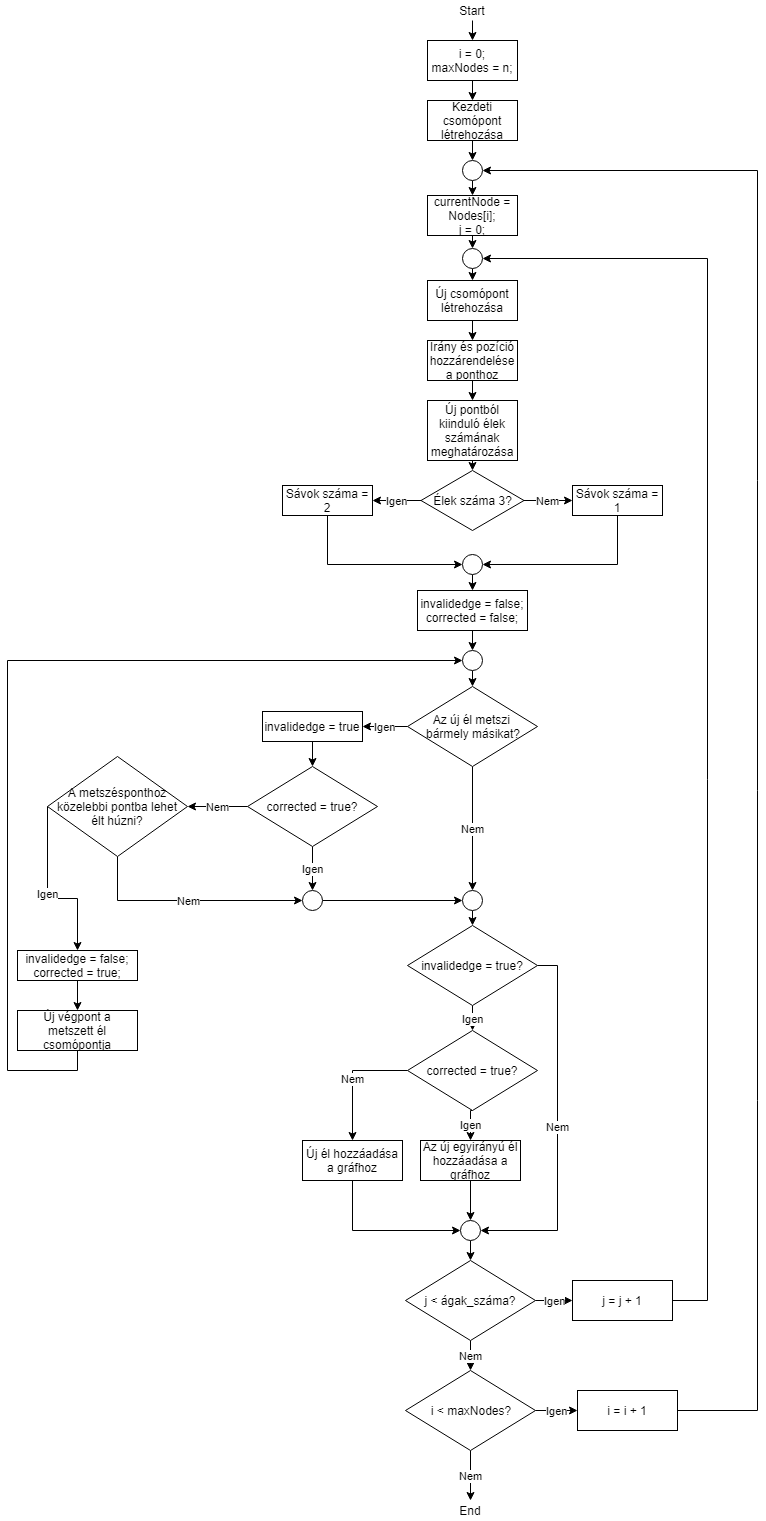
\includegraphics[keepaspectratio,scale=0.45]{folyamat.png}
\caption{A generálás lépéseinek egyszerűsített folyamatábrája}
\label{fig:flowchart}
\end{figure}
\subsection{Generáló algoritmus}
A csomópontok generálása a következőképpen történik:
\begin{enumerate}
\item A kiválasztott csomópont kap egy véletlenszerű irányt, észak, dél, kelet, vagy nyugat értékében
\item Ha a kapott érték megegyezik azzal az iránnyal amerre a csomópont szülője van, vagy már indult arra belőle él, újat kap
\item A kiválasztott iránynak megfelelő véletlen generált X és Y koordinátákat kap
\item A kapott koordinátákból alkotott csomópont felkerül a gráfra
\item Ha a jelenlegi csomópontból még kell éleket indítani, akkor kezdődik előröl
\end{enumerate}
Az előbbiekben említett X és Y koordinátát kissé pontosítanám. Ha a csomópontot nyugat vagy kelet irányba generáljuk, az X koordináta értéke a jelenlegi pont X koordinátája, hozzáadva egy
előre definiált értékek közötti véletlen szám. Az Y koordináta ilyenkor egy minimális eltérés az út fekvésében, hasonlóan generálódik, de lényegesen alacsonabb véletlen számot kap. Ez
tulajdonképpen a valóságban is látható "tökéletlenségekre" vezethető vissza, ugyanis a legtöbb esetben ott sem teljesen merőleges egymásra kettő út. Az észak és dél irányba induló pontok 
esetén ugyan ez az eljárás, csak a két koordináta szerepe felcserélődik.
Fontos viszont az is, hogy a középponttól távolodva átlagosan kevesebb elágazása legyen egy csomópontnak, ezért ehhez felhasználható annak gráfbeli szintje. Minden csomópontról eltárolódik 
annak szintje (szülő szintje + 1), ami befolyásolja az elágazások számát. Egy másik probléma az, hogy az így generált élek gyakran metszhetik egymást, amely az aluljárók és a hídak hiányában 
itt nem megengedett, ezért utolsó lépésnek ellenőrizni kell hogy az új él metszi-e bármely meglévő élek közül akár az egyiket is, és ha igen akkor nem kerülhet fel a gráfra. Az él viszont hozzáadható 
az eredetileg kijelölt csomóponthoz legközelebbi csomóponttal történő helyettesítéssel, feltéve ha így nem történik létező út metszése.
A buszmegállók elhelyezésével kapcsolatban a következő feltételeket
adtam:
\begin{itemize}
\item A legcélszerűbb a hálózat két, egymástól távol lévő, a gráf mélyebb szintjein elhelyezkedő pont közötti út létrehozása
\item Az útvonalnak érintenie kell a középpontot, a gráf 0. szintjét
\item Lehető legkevesebbszer érintse többször ugyan azt a csomópontot
\end{itemize}
Ennek érdekében először kijelölöm az út egyik végét, mint megállót. Ezek után keresek egy utat a gráf 0. szintjéhez, melyen legfeljebb minden második csomópontot kijelölöm megállónak. A középpont 
elérése után kijelölöm a második végpontot, mely a középponttól az eddigi iránynak ellentétesen, a gráf mélyebb szintjei közül kell lennie. Az ehhez a középpontból vezető úton, az utóbbihoz hasonló 
eljárással kijelölök megállókat. Az utak sávszámának meghatározására a gráfbeli mélységüket használom. A magasabb szinten lévő élek nagyobb valószínűséggel lesznek többsávosak. Ez a generálás végén választódik
ki. Az egyirányú utak kijelölése is a folyamat legvégén történik. Ennek az oka magából az utak jellegéből adódik, ugyanis egyirányú út nem végződhet zsákutcában, és nem is zárhatja el a hálózat egy részét a többi elől. Éppen ezért egy olyan részgráfot kell találni amely Hamilton-kört alkot, amelyen egy részgráfot már nyugodtan egyirányúvá lehet tenni.
\subsection{Az egyirányú út}
Egy könnyű módszer annak megoldására, hogy mely utak lehetnek egyirányúak az lenne, ha a generálás során egymást metszett utakból kialakult éleket jelölöm el egyirányúnak. Ezek az élek ugyanis biztos hogy egy létező Hamilton-út részei, mivel az eredetileg fagráfnak megfelelő úthálózat bármely két csomópontja közé húzott él Hamilton-utat ad.
\Section{Alapelemek megjelenítése HTML Canvas segítségével}
\subsection{Fejlesztői környezet felállítása}
Az algoritmus működését, eredményét egy HTML Canvas objektumon szemléltetem. Magát a kódot JavaScript-ben írtam, annak ECMAScript 6-os verziójában. Fejlesztői környezetnek A JetBrains által készített WebStormot használtam. Először is 
létrehoztam egy HTML fájlt, ahol a body tag-en belül elhelyeztem a canvas elemet. Erre az elemre JavaScriptből a HTML-ben megadott id-je alapján lehet hivatkozni. Ezután létrehoztam egy JavaScript fájlt, melyben egy (document).ready() szintaktikában 
elhelyezett függvényhívással indítom a generálást. A (document).ready() a jQuery függvénykönyvtárnak része. Azért szükséges ebben az esetben, mert ameddig a html fájl nem töltött be teljesen, a script nem futtatható mert a canvas elemre nem létezne 
semmilyen referencia. Ez a részlet biztosítja hogy csak akkor kezdődjön a script futtatása, ha a HTML documentum teljesen betöltött. A js fájlban globálisan eltárolom egy változóba a canvasre mutató referenciát, majd egy másik váltózóba lekérem ennek a kontextusát.
\subsection{Létrehozott osztályok}
\subsubsection{Node}
A gráfon egy csomópontot leíró objektum. Egy konstruktort tartalmaz, amely beállítja az osztály 6 adattagjának értéket. Ezek az adattagok a következőek:
\begin{itemize}
\item x: A csomópont X koordinátája
\item y: A csomópont Y koordinátája
\item branches: Hányfelé kell tovább ágaztatni a csomópontot
\item level: A gráf hanyadik szintjén helyezkedik el a csomópont
\item connectedFrom: Milyen irányból lett kiterjesztve a csomópont
\item parentNodeIndex: A gráfban lévő csomópontokat tartalmazó vektoron belül ezen csomópont szülőjének indexe
\end{itemize}
\subsubsection{Edge}
A gráfon egy él leírására szolgáló objektum. Egy konstruktort tartalmaz, amely inicializálja 4 adattagját. Ezek az alábbiak:
\begin{itemize}
\item from: Az a csomópont, ahonnan az él kezdődik
\item to: Az a csomópont, amiben az él végződik
\item lanes: Az él által jelölt úton hány sáv van
\item oneway: Logikai változó, az út egyirányú-e vagy sem
\end{itemize}
\subsubsection{Graph}
Magát a gráfot leíró objektum, mely tartalmaz 2 függvényt annak canvas-on történő kirajzolására. Paraméter nélküli konstruktora 2 adattagját inicializálja üres értékkel. Adattagjai és függvényei a következők:
\begin{itemize}
\item Nodes: A csomópontokat tartalmazó vektor
\item Edges: Az éleket tartalmazó vektor
\item drawAllNodes: Függvény, mely végig iterál a Nodes vektoron, és mindegyik elemére meghívja a kirajzoló függvényt
\item drawAllEdges: Függvény, végig iterál az Edges vektoron, egyirányú út esetén nyilat rajzol, ellenkező esetben egyenes vonalat
\end{itemize}
\subsection{Segédfüggvények}
\subsubsection{intersects}
Ez a függvény arra szolgál, hogy kiszámítsa két él metszi-e egymást. Ehhez két paramétert vár, edge1 és edge2 néven. Visszatérési értéke logikai típusú.
Működésében a két szakaszból egyeneseket képez, majd ezek alapján az X = v1 + lambda*d1, X = v2 + gamma *d2 egyenletrendszer mátrixának kiszámolja a determinánsát. Ha ez 0, a két szakasz nem metszi egymást.
Ellenkező esetben megnézi az egyenletrendszerben szereplő gamma és lambda értékeket, azaz a két egyenes mentén az irányvektor hányszorosát kell venni hogy elérkezzünk a ponthoz. Ha ez nem 0 és 1 közé esik, a metszéspont nincs a szakaszon belül.
\begin{cpp}
function intersects(edge1,edge2) {
    let det, gamma, lambda;
    det = (edge1.to.x - edge1.from.x) * (edge2.to.y - edge2.from.y) - 
    (edge2.to.x - edge2.from.x) * (edge1.to.y - edge1.from.y);
    if (det === 0) {
        return false;
    } else {
        lambda = ((edge2.to.y - edge2.from.y) * (edge2.to.x - edge1.from.x)
         + (edge2.from.x - edge2.to.x) * (edge2.to.y - edge1.from.y)) / det;
        gamma = ((edge1.from.y - edge1.to.y) * (edge2.to.x - edge1.from.x)
         + (edge1.to.x - edge1.from.x) * (edge2.to.y - edge1.from.y)) / det;
        return (0 < lambda && lambda < 1) && (0 < gamma && gamma < 1);
    }
}
\end{cpp}
\subsubsection{distance}
Két csomópont közötti távolság kiszámítására szolgáló függvény. Ehhez a két vektor által meghatározott szakasz hosszát számolja ki pitagorasz tétellel. Ezzel az eredménnyel tér vissza.
\subsubsection{maxBranchesReached}
Ezzel a függvénnyel megmondható hogy egy adott csomópontba már lett-e 4 él húzva. A függvény paramétereiként megkapja a keresett csomópontot, a gráfot, és a jelenleg kiterjesztés alatt álló csomópont gráfbeli indexét. Amennyiben a gráfban megtalált csomópont branches értéke kisebb mint 3, akkor növeli 1-el és hamis értékkel tér vissza, azaz még nem volt 4 él húzva. Ellenkező esetben igaz értéket ad.
\subsubsection{getBranchCount}
Ez a függvény egy egész számot kap paraméterként, mely egy csomópont gráfbeli mélységére utal. Ez alapján a szám szerint visszaadja hogy mennyi irányba ágazzon el az adott csomópont. Első szinten 80\% az esélye hogy 4 irányban ágazik el, ez szintenként 20\%-al csökken. Ha nem 4 irányban ágazik el, véletlenszerűen generált számot ad vissza 0 és 2 között, mivel a csomópont szülőjéhez vezető élt ilyenkor nem számoljuk.
\subsubsection{findMaxLevelNodes}
A gráf legmélyebb szintjén lévő csomópontok megtalálására szolgáló függvény. Paraméterként megkapja a gráfot. Első lépésben beállítja a max értéket a gráf első csomópontjának szintjére, és inicializálja a maximális mélységben elhelyezkedő csomópontok vektorát. Ezután maximum kereséssel beállítja max értéket. Majd a gráf Nodes vektorán végig iterálva hozzáadja az ezen max értéknek megfelelő mélységű csomópontokat az eredmény vektorhoz. Végül ezzel a vektorral tér vissza.
\subsubsection{DrawBStops}
Buszmegálló rajzolására használt függvény. Egy csomópontot kap paraméterként. A kontextust felhasználva felrajzolja a canvasra egy zöld négyzet formájában. Visszatérési értéke nincs.
\subsubsection{makeBusStops}
Ez a függvény szolgál a buszmegállók elhelyezésére. Egyelőre csak a hozzávetőleges helyüket jelöli, nem az él közepére teszi a helyüket, hanem a csomópontokra. Paraméterként megkapja a gráfot. Előszőr meghívja a findMaxLevelNodes függvényt, ebből a kapott értéket eltárolja egy változóba. 

Kijelöl az útvonal kezdetének az előbb kapott vektorból egy véletlenszerű elemet. Ezt felrajzolja a DrawBStops függvénnyel. Ezután végig iterál a maximum mélységű tömbökön, maximum keresést végezve a kiindulási ponttól mért távolságot illetően. Ehhez a distance függvényt használja. Ha megvan a végpont azt is felrajzolja. 
Ezután elindul a kiindulási ponttól, sorra véve a csomópontok szüleit. Minden buszmegálló kirajzolása után kap egy véletlen értéket, amely megmondja hogy hány csomópont után kell rajzolnia mégegyet. Ha eljutott a gráf kezdőpontjáig megcsinálja ugyan ezt az út végpontjától is. Visszatérési értéke nincs.
\subsubsection{drawCanvasNode}
Egy paraméterként megkapott csomópont koordinátáinak megfelelő helyre négyzetet rajzol a canvasre.
\subsubsection{drawCanvasEdge}
Egy élt kap meg paraméterként, melynek kezdő és végpontjai között egyenes vonalat húz a canvasre.
\subsection{A generáló függvény}
A generálás kódjának fő része ebben a függvényben van. Ez egy paraméter nélküli függvény, visszatérési érték nélkül. A következőkben vázolom a működését. 

Először inicializálja a gráfot az osztály példányosításával, majd kijelöli a kezdő csomópontot, annak paramétereit beállítva fix értékekre, tehát 4 elágazású lesz, az 1000,500 koordinátákon. 

Ezután egy for ciklussal végig iterál a csomópontokat tároló vektoron, minden csomóponton kezdetben megadja a connectedFrom értéket, tehát hogy az adott csomópont melyik irányból lett kiterjesztve. 

Ha ez megvan, újabb ciklus kezdődik, mely a csomópont elágazásait terjeszti ki egyesével. Ezen belül megkapja minden iterációban a kiterjesztés irányát, az új csomópont elágazásainak számát a getBranchCount függvénnyel, valamint az új élen lévő sávok száma is kiszámítódik. Ilyenkor már létezik az új él és csomópont mint objektum, következő lépésben megnézi hogy az új él metszi-e bármely meglévő élt. Ez egy szimpla iteráció az éleket tartalmazó vektoron, az intersects függvény segítségével eldönti hogy történt-e metszés.

Amennyiben volt metszés, de az élt be lehetett húzni a metszett élnek a metszésponthoz közelebb álló csomópontjához, az új él megmarad, és egyirányú lesz, a csomópontot pedig elvetjük. Ha nem lehetett behúzni, vagy még így is történt metszés, akkor mindkettőt elvetjük. Ezen vizsgálat után az új él és csomópont amennyiben valamelyik is alkalmas maradt, hozzáadásra kerülnek a gráfbeli vektorhoz.

Miután a kellő mennyiségű csomópont ki lett terjesztve, a függvény meghívja a gráfon belüli drawAllNodes és drawAllEdges függvényeket, majd végül a makeBusStops függvényt. Ezzel kész a generálás, az elemek felkerültek a canvasre.
\begin{figure}[H]
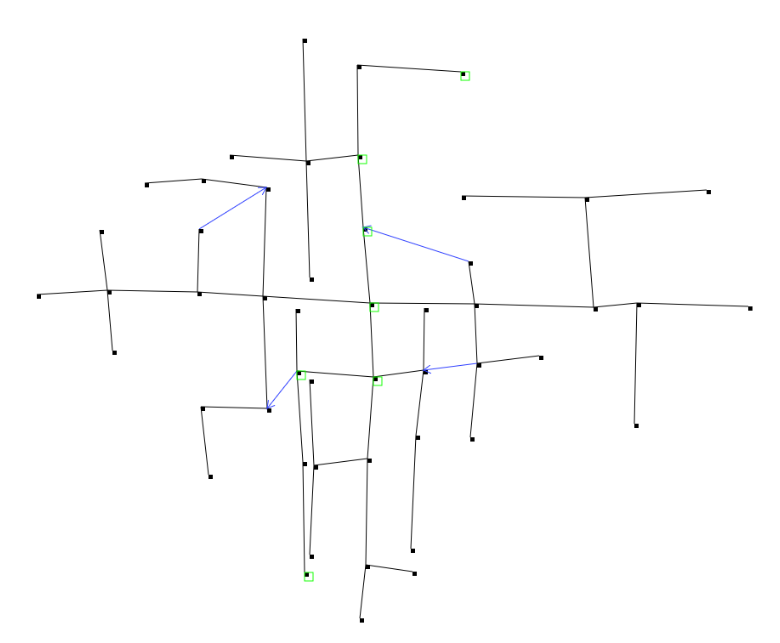
\includegraphics[width=\linewidth]{graph.png}
\caption{Kép a generáló algoritmus eddigi eredményéről}
\label{fig:graph}
\end{figure}
\Section{Az algoritmus implementálása Unity-ben}
Mivel a szimulációt a Unity Enginel fogom elkészíteni, első lépésben az előbbi JavaScript implementációt ki kell bővíteni. Ez főleg a kirajzoló függvények átírását fogja jelenteni, amelyben 2D canvas helyett most már 3D-s megjelenítésben kell gondolkozni, de ezen kívül a C\# programnyelvre való áttérés miatt lehetnek még minimális változtatások.
\begin{figure}[H]
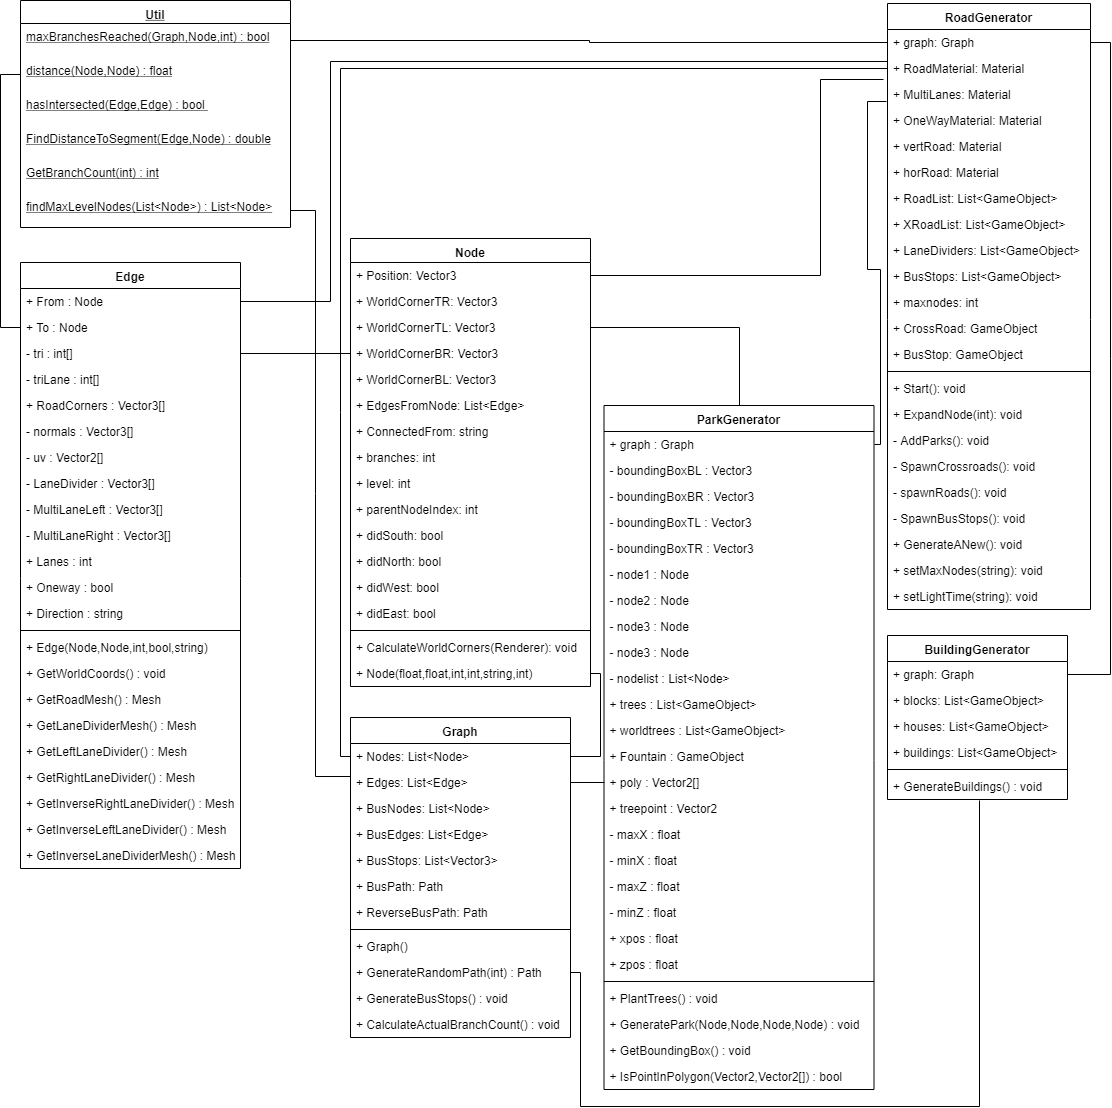
\includegraphics[scale=0.45,keepaspectratio]{generateuml.png}
\caption{A generálásban résztvevő osztályok UML osztálydiagramja}
\label{fig:genuml}
\end{figure}
\subsection{Osztályok}
\subsubsection{Util}
Létrehoztam egy Util nevű statikus osztályt, melynek fő célja az lenne hogy külön osztályba összegyűjti az összes használt matematikai Segédfüggvényt. Ebbe az osztályba került bele a maxBranchesReached, a distance, az intersects mostmár hasIntersected néven, a getBranchCount, valamint a findMaxLevelNodes függvények. 

Továbbá bővült egy újab fügvénnyel, a FindDistanceToSegment-el. Ez a függvény paraméterként egy élt és egy csomópontot vár. Visszatérési értékként a csomópont és a szakasz közötti legrövidebb távolságot adja.
\subsubsection{Node}
Ez az osztály az eredeti implementációhoz nagy mértékben hasonló. Egy lényeges különbség, hogy a csomópont pozícióját egy Vector3 típusú adattagban tárolom. Ez a típus 3 float típusú koordinátát tárol, az x,y, és z koordinátákat.

Hozzáadtam valamint 5 új adattagot, amelyek közül 4 a csomóponthoz tartozó objektum négy sarkát jelőlik. Ezek az adattagok Vector3 típusúak, kiszámításukra az osztályon belül elhelyeztem egy CalculateWorldCorners függvényt, melynek paraméterül meg kell adni a létező csomópont objektum Renderer komponensét.

Az ötödik új adattag egy Edge lista, mely a csomópontból kiinduló éleket tartalmazza, nem beleértve az ide érkezőket.

A CalculateWorldCorners függvény a következő képpen használja fel a renderert: a renderer objektum képes visszaadni a hozzá tartozó 3D mesht behatároló téglatestet. Ennek a téglatestnek lekérdezhető a maximum és minimum értéke, mely rendszerint a jobb felső és a bal alsó sarkát adja vissza. Ezen két pont tudatában kiszámítható a maradék két sarok is, a koordináták vegyes felhasználásával.
\begin{cpp}
public void CalculateWorldCorners (Renderer renderer)
        {
            WorldCornerTR = renderer.bounds.max;
            WorldCornerTL = new Vector3(renderer.bounds.min.x, 
            0.1f, renderer.bounds.max.z);
            WorldCornerBL = renderer.bounds.min;
            WorldCornerBR = new Vector3(renderer.bounds.max.x,
            0.1f, renderer.bounds.min.z);
        }
\end{cpp}
\subsubsection{Edge}
Ez az osztály esett át a legnagyobb átalakításon, ugyanis az utat ábrázoló mesht dinamikusan kell kirajzolni, amelyhez először el kell végezni néhány számítást.

A konstruktora változatlan maradt, viszont az osztály rengeteg adattaggal bővült. Először is a RoadCorners Vector3 típusú tömbbel, amely az útszakasz négy sarkának koordinátáit tárolja. A mesh megalkotásához szükséges a poligont alkotó háromszögek megadása, erre létrehoztam egy egész típusú tri tömböt.

Szintén hasonlóan, az úton jelen lévő felezővonalak, sávelválasztó vonalak jelölésére is szükség van egy objektumra. A felezővonal sarkait a LaneDivider tömbbe, a bal és jobb oldali sávelválasztó sarkait pedig a MultiLaneLeft és MultiLaneRight Vector3 típusú tömbben tárolom. Ezeknek a válaszvonalaknak külön háromszög tömböt is deklaráltam triLane néven.

A meshez szükséges még normálvektorokat tartalmazó, illetve uv tömböket is bevezettem.

Az osztály új metódusokkal bővült, ezek közül első a GetWorldCoords void típusú paraméter nélküli metódus. Ez a metódus annak függvényében, hogy a Direction adattagban milyen irány van megadva, kiszámolja az általa összekötött csomópontok sarkai alapján az útszakasz sarkainak koordinátáit.
\begin{cpp}
case "north":
                    RoadCorners[0] = From.WorldCornerTL;
                    RoadCorners[1] = From.WorldCornerTR;
                    RoadCorners[2] = To.WorldCornerBL;
                    RoadCorners[3] = To.WorldCornerBR;
                    LaneDivider[0] = ((RoadCorners[0] + 
                    RoadCorners[1]) / 2) + Vector3.up * 5;
                    LaneDivider[1] = ((RoadCorners[0] + 
                    RoadCorners[1]) / 2) + Vector3.up * 10;
                    LaneDivider[2] = ((RoadCorners[2] +
                     RoadCorners[3]) / 2) + Vector3.up * 5;
                    LaneDivider[3] = ((RoadCorners[2] + 
                    RoadCorners[3]) / 2) + Vector3.up * 10;
                    if (Lanes == 2)
                    {
                        MultiLaneLeft[0] = ((RoadCorners[0] + 
                        Vector3.up * 5) + LaneDivider[0]) / 2;
                        MultiLaneLeft[1] = ((RoadCorners[0] + 
                        Vector3.up * 10) + LaneDivider[1]) / 2;
                        MultiLaneLeft[2] = ((RoadCorners[2] + 
                        Vector3.up * 5) + LaneDivider[2]) / 2;
                        MultiLaneLeft[3] = ((RoadCorners[2] +
                        Vector3.up * 10) + LaneDivider[3]) / 2;
                        MultiLaneRight[0] = ((RoadCorners[1] + 
                        Vector3.up * 5) + LaneDivider[0]) / 2;
                        MultiLaneRight[1] = ((RoadCorners[1] + 
                        Vector3.up * 10) + LaneDivider[1]) / 2;
                        MultiLaneRight[2] = ((RoadCorners[3] + 
                        Vector3.up * 5) + LaneDivider[2]) / 2;
                        MultiLaneRight[3] = ((RoadCorners[3] + 
                        Vector3.up * 10) + LaneDivider[3]) / 2;
                    }
                    break;
\end{cpp}
Példa esetként, ha észak felé tart az út, akkor a kiindulási pont bal és jobb felső, a célpont bal és jobb alsó koordinátáira lesz szükség.

Ha az út két sávos, ezen sarkok alapján kiszámolja a felező- és sávelválasztó vonalak sarkait. Ezek megjelenésével nem kell foglalkozni, csak jelző értékkel rendelkeznek a járművek számára, ezért az útszakasz felett foglalnak helyet, egész pontosan 5 egységnyi értékkel felette.

Ezek után beállítja a tri és triLane értékeit, azaz hogy a háromszögek megalkotásához milyen sorrendbe járja be az adott pontokat.


A GetRoadMesh metódus maga az utat reprezentáló Mesh objektummal tér vissza. Paraméter nélküli metódus. Első lépésben meghívja a GetWorldCoords függvényt, ezzel beállítva az út sarkainak értéket. Majd létrehoz egy új Mesh objektumot, melynek csúcsait beállítja az előbb kiszámolt pontokra, háromszögek értéket pedig a tri tömbre. A normálvektorok itt nem kapnak nagy jelentőséget, Z tengely szerinti negatív egyenes értéket adtam nekik. Az uv koordinátákat szimplán a mesh négy sarkának jelöltem el.
\begin{cpp}
public Mesh GetRoadMesh()
        {
            GetWorldCoords();
            Mesh mesh = new Mesh();
            mesh.vertices = RoadCorners;
            mesh.triangles = tri;
            normals[0] = -Vector3.forward;
            normals[1] = -Vector3.forward;
            normals[2] = -Vector3.forward;
            normals[3] = -Vector3.forward;
            mesh.normals = normals;
            uv[0] = new Vector2(0, 0);
            uv[1] = new Vector2(1, 0);
            uv[2] = new Vector2(0, 1);
            uv[3] = new Vector2(1, 1);
            mesh.uv = uv;
            return mesh;
        }
\end{cpp}
A GetLaneDividerMesh, GetLeftLaneDivider, valamint a GetRightLaneDivider metódusok az előbbivel hasonló módon funkcionálnak, csak a csúcsok halmaza változik.

Ám ezekkel a vonalakkal kapcsolatban szükség volt létrehoznom három Inverse metódust is, a GetInverseLeftLaneDivider, GetInverseRightLaneDivider, és a GetInverseLaneDividerMesh függvényeket. Erre az a magyarázat, hogy ezek alapvetően síkok, azaz a hátlapjaik nem láthatóak. 

Bár a Unity tartalmaz megoldást ütközők konvexé alakítására, ez ebben az esetben nem mindig működik, mert gyakran a válaszvonal négy csúcsai koplanáris pontok. Ezért a következő megoldást választottam: a létrehozott síkokkal megegyező pozícióban létrehozom a síkok ellentétes irányba néző változatát. Ezt a feladatot látják el ezek az inverse metódusok, melyek az adott háromszög tömböt visszafelé járják be.

\subsubsection{Graph}
A gráfot leíró osztály bővült néhány új adattaggal. 

Külön Node és Edge listában tartalmazza mostmár a buszok útvonalát leíró csomópontokat és éleket. A buszmegállok koordinátái tárolására egy Vector3 típusú listát is bevezettem.

Továbbá ebben az osztályban tárolom a buszok számára kirendelt útvonalat is, melyet egy Path nevű osztállyal írok le. Ezt a későbbiekben részletezném a szimulációval kapcsolatban.

Az osztály konstruktora üres listával inicializálja az összes adattagot.

Egy új metódus került az osztályba, a GenerateRandomPath. Ennek egy egész szám típusú paramétert kell megadni, ez lesz az útvonal maximális hossza. A metódus visszatérési értéke Path típusú, ez fogja tartalmazni az útvonal adatait.

Működésében egy Node és egy Edge listában tárolja el az útvonal által bejárt csomópontokat és éleket. Először választ egy véletlenszerű csomópontot, majd a csomópontból kiinduló élek közül választ egyet, és az él túlsó végén lévő csomóponthoz megy tovább. Ezt addig folytatja, amíg el nem éri a megadott maximális úthosszat, vagy ameddig már nem lehet tovább menni egy adott csomópontból. Végül a Node és Edge listát felhasználva visszadja a Path objektumot.
\begin{cpp}
while(currentsize < length && nextnode.EdgesFromNode.Count > 1)
            {
                Edge nextedge = nextnode.
                EdgesFromNode[Random.Range(0, nextnode.EdgesFromNode.
                Count)];
                if(nextedge.From != previousNode && nextedge.To != 
                previousNode)
                {
                    previousNode = nextnode;
                    nextnode = nextnode == nextedge.From ? nextedge.To : 
                    nextedge.From;
                    edges.Add(nextedge);
                    nodes.Add(nextnode);
                    currentsize++;
                }
                
            }
\end{cpp}

A GenerateBusStops metódusban történt pár változtatás. Ezt is úgy írtam meg, hogy a Path objektumot használja, ezért a metódus az osztályon belüli két busz útvonalat leíró adattag értékét állítja be.

Működésében nagyjából azonos, egy fontos változtatással, miszerint a megállók elhelyezése közben bejárt csomópontokat és éleket eltárolja listában. Az útvonal vége felőli bejárt utat megfordítás után hozzáadom a kiindulás felőli úthoz, ez adja a busz teljes útvonalát.

Ezt az útvonalat megfordítom teljes egészében, így megkapom a buszok útvonalát ellentétes irányban. Mindkettő útvonal tárolódik a végén.
\begin{cpp}
nodesfromEnd.RemoveAt(nodesfromEnd.Count - 1);
nodesfromEnd.Reverse();
BusNodes.AddRange(nodesfromEnd);
edgesfromEnd.Reverse();
BusEdges.AddRange(edgesfromEnd);
this.ReverseBusPath = new Path(BusNodes, BusEdges);
BusEdges.Reverse();
BusNodes.Reverse();
this.BusPath = new Path(BusNodes, BusEdges);
\end{cpp}
A CalculataActualBranchCount metódusra azért volt szükség, mert generálás után a csomópont branches adattagja nem minden esetben reflektálja a hozzá tartozó tényleges élek számát, például ha az egyik kiterjesztése érvénytelen volt. Ez a metódus megszámolja ténylegesen hány él indul és/vagy érkezik az adott csomópontba, és ez alapján beállítja a branches értékét.
\begin{cpp}
public void CalculateActualBranchCount()
        {
            foreach (Node n in Nodes)
            {
                n.branches = 0;
                foreach(Edge e in Edges)
                {
                    if((e.To.Position == n.Position) || 
                    (e.From.Position == n.Position && !e.Oneway))
                    {
                        n.branches++;
                    }
                }
            }
        }
\end{cpp}
\subsubsection{BuildingGenerator}
Ez az osztály felelős az utak menti épületek elhelyezéséért. Adattagjai közé tartozik az úthálózatot reprezentáló Graph típusú graph, a kertes- és blokkházak sablonjait tartalmazó blocks és houses GameObject típusú lista, valamint a legenerált épületeket tartalmazó buildings lista.

Egyetlen metódusa van, a GenerateBuildings paraméter nélküli, void visszatérésű metódus. Ebben a metódusban történik a generálás több lépésben.
Első lépésben megnézi, van-e legalább 30 csomópont a gráfban. Hogyha igen, akkor a gráf azon szintjein, amelyek nagyobbak, mint a csomópontszám 1/25-e, blokkházakat helyez el, ahol kisebb ott kertesházakat.
Hogyha kevesebb mint 30 csomópontból áll a gráf, akkor mindenhova kertesházat fog elhelyezni. Az épületek pozíciójának kijelölésére kiszámolja az adott élet reprezentáló vektort, annak vég- és kezdőpontjának különbségével. Ezután kiszámol egy ezen vektorra merőleges vektort, mely az él vektorának és az y tengelyt reprezentáló vektornak vektoriális szorzata. Ennek kiszámítására tartalmaz a Vector3 struktúra egy Cross nevű metódust. Az út vektorát 9 részre osztom fel, ezen részek hosszát egy buildingslot nevű vektor tárolja.
Ezen adatok kiszámítása után egy for cikluson belül elhelyezi az épületeket. A ciklusváltozó kezdeti értéke megegyezik a buildingslot vektorral, amely minden iteráció után a buildingslot értékével nő. Kilépési feltételként adtam azt, hogy a ciklusváltozóban tárolt vektor hosszának  nagyobbnak kell lennie, mint az élt jelölő vektor hosszánál 20 egységgel kisebb vektor. Ezzel elkerülöm azt, hogy útkereszteződéshez túl közel kerüljön egy épület. Mielőtt elhelyezne egy épületet, megnézi hogy az adott területen megadott területen belül létezik-e valamilyen más objektumhoz tartozó Collider komponens. Ez annak érdekében kell, hogy ne kerüljön fa épületen belülre, illetve ne legyen két épület túl közel egymáshoz.

A kertesházak elhelyezéséért felelős blokk a következő, ezzel működésben megegyezik a blokkházaké is, csupán a vektorok méretében van különbség:
\begin{cpp}
Vector3 theRoad = e.To.Position - e.From.Position;
Vector3 buildingslot = theRoad / 10f;
Vector3 side = Vector3.Cross(theRoad, Vector3.up).normalized;
for (Vector3 offset = buildingslot; offset.magnitude < theRoad.
magnitude - 20f; offset += buildingslot)
{
    if (!Physics.CheckBox(e.From.Position + offset + side * 14f + 
    Vector3.up * 6f, new Vector3(5f, 5f, 5f)))
    {
        buildings.Add(Instantiate(houses[Random.Range(0, 2)], e.
        From.Position + offset + side * 14f, Quaternion.identity));
    }
    if (!Physics.CheckBox(e.From.Position + offset - side * 14f + 
    Vector3.up * 6f, new Vector3(5f, 5f, 5f)))
    {
        buildings.Add(Instantiate(houses[Random.Range(0, 2)], e.
        From.Position + offset - side * 14f, Quaternion.identity));
    }
\end{cpp}
\subsubsection{ParkGenerator}
A ParkGenerator osztály tartalmazza a fák és a parkok generálásáért felelős metódusokat. Adattagjai közé tartozik a gráf, a park négy sarkát jelölő Node típusú csúcspontok, valamint Vector3 típusú koordináták, ezen négy pont tárolására alkalmas Node lista, valamint a koordináták tárolására alkalmas Vector2 tömb, a generált fák tárolásáért felelős GameObject típusú worldtrees tömb, és végül a fák sablonjait tartalmazó trees GameObject típusú lista.

Az osztály PlantTrees metódusa  véletlenszerű pozíciókban fákat helyez el, a gráfot befoglaló négyzet területén belül. Első lépésben kiszámolja ezen négyzet négy sarkát, linq függvények segítségével. Ezután a gráf csomópontszámának ötszörösének megfelelő mennyiségű fát helyez el.
\begin{cpp}
public void PlantTrees()
    {
        float minx = graph.Nodes.OrderByDescending(
        x => x.Position.x).LastOrDefault().Position.x;
        float maxx = graph.Nodes.OrderByDescending(
        x => x.Position.x).FirstOrDefault().Position.x;
        float minz = graph.Nodes.OrderByDescending(
        x => x.Position.z).LastOrDefault().Position.z;
        float maxz = graph.Nodes.OrderByDescending(
        x => x.Position.z).FirstOrDefault().Position.z;
        for (int i = 0; i < 5 * graph.Nodes.Count; i++)
        {
            xpos = Random.Range(minx, maxx);
            zpos = Random.Range(minz, maxz);
            treepoint = new Vector2(xpos, zpos);
            if (!Physics.CheckBox(new Vector3(treepoint.x, 6f, 
            treepoint.y), new Vector3(5f, 5f, 5f)))
            {
                worldtrees.Add(Instantiate(trees[Random.Range(0, 3)], 
                new Vector3(treepoint.x, 0.1f, treepoint.y), 
                Quaternion.identity));
            }
        }
    }
\end{cpp}
A GetBoundingBox függvény szerepe a kapott csomópontok alapján meghatározni hogy azok közül melyik pont a park melyik sarkát jelenti. Így megkapjuk a bal alsó és felső, valamint jobb alsó és felső sarkát a parknak.
\begin{cpp}
private void GetBoundingBox()
    {
        maxX = nodelist.OrderByDescending(
        x => x.Position.x).FirstOrDefault().Position.x;
        minX = nodelist.OrderByDescending(
        x => x.Position.x).LastOrDefault().Position.x;
        maxZ = nodelist.OrderByDescending(
        x => x.Position.z).FirstOrDefault().Position.z;
        minZ = nodelist.OrderByDescending(
        x => x.Position.z).LastOrDefault().Position.z;
        boundingBoxBL = new Vector3(minX, 0.1f, minZ);
        boundingBoxBR = new Vector3(maxX, 0.1f, minZ);
        boundingBoxTL = new Vector3(minX, 0.1f, maxZ);
        boundingBoxTR = new Vector3(maxX, 0.1f, maxZ);
    }
\end{cpp}
Az IsPointInPolygon függvény két paramétert kap, egy Vector2 típusú pontot, valamint egy Vector2 tömböt amely tartalmazza egy poligon pontjait. Visszatérési értéke igaz, hogyha a pont benne van a poligonban, hamis hogyha nincs. Ennek meghatározására megnézi a poligon összes élét jellemző szakaszra, hogy a pont ezen szakasz végpontjai közé esik-e, valamint ha igen, akkor a szakasz megfelelő oldalán van-e.
\begin{cpp}
public bool IsPointInPolygon(Vector2 point, Vector2[] polygon)
    {
        int polygonLength = polygon.Length, i = 0;
        bool inside = false;
        float pointX = point.x, pointY = point.y;
        float startX, startY, endX, endY;
        Vector2 endPoint = polygon[polygonLength - 1];
        endX = endPoint.x;
        endY = endPoint.y;
        while (i < polygonLength)
        {
            startX = endX; startY = endY;
            endPoint = polygon[i++];
            endX = endPoint.x; endY = endPoint.y;
            //
            inside ^= (endY > pointY ^ startY > pointY)
                      && ((pointX - endX) < (pointY - endY) * 
                      (startX - endX) / (startY - endY));
        }
        return inside;
    }
\end{cpp}

A parkok generálását a GeneratePark függvény végzi. Paraméterként megkapja a parkot leíró négy csomópontot. Ezen négy csomópont alapján meghatározza a park négy sarkát a GetBoundingBox függvénnyel. Miután ez megvan, egy for ciklusban elhelyez 100 darab fát a park területén belül véletlenszerű pozícióban. Az objektumok elhelyezése előtt megnézi, hogy ütközne-e bármely más objektummal, hogyha igen akkor új pozíciót kap. Végül hasonló módszerrel elhelyez egy darab szökőkutat is a parkban.
\begin{cpp}
do
        {
            xpos = Random.Range(minX, maxX);
            zpos = Random.Range(minZ, maxZ);
            treepoint = new Vector2(xpos, zpos);
        } while (!IsPointInPolygon(treepoint, poly) || Physics.
        CheckBox(new Vector3(treepoint.x, 6f, treepoint.y), 
        new Vector3(5f, 5f, 5f)));
        worldtrees.Add(Instantiate(Fountain, new Vector3(treepoint.x, 
        0.1f, treepoint.y), Quaternion.identity));
\end{cpp}
\subsubsection{RoadGenerator}
Többek között ebbe az osztályba került a fő generáló függvény, valamint a kirajzolásért felelő függvények.

Adattagjai közé tartozik maga a gráf, mint Graph típus, külön Material típus három féle útra (egy sávos, két sávos, egyirányú), négy GameObject lista, melyek az útszakaszok, az útkereszteződések, a választóvonalak, és a buszmegállók tárolására vannak, valamint egy sablon objektum elhelyezésére alkalmas CrossRoad és BusStop GameObject típusú adattagok.

Az osztályon belüli Start metódus az ezen osztály komponensként tartalmazó objektum létrejötte utáni legelső képkockában fut le, pontosan egyszer.

Ebben a metódusban először elhelyezem a kezdeti csomópontot, majd ameddig kevesebb csomópont létezik mint a megadott maximum, az ExpandNode metódussal kiterjesztem a soron következő csomópontot.

Ha ez megtörtént, újra számoltatom a csomópontok elágazásainak számát a gráfon belüli CalculataActualBranchCount metódussal, majd meghívom a SpawnCrossroads, spawnRoads, a gráfon belüli GenerateBusStops, majd a SpawnBusStops metódusokat a csomópontok, útszakaszok, és a buszmegállók kirajzolásához. Ha ez megtörtént, beállítom a BuildingGenerator és a ParkGenerator komponensek graph értékét az ebben az osztályban eltárolt gráfra, majd végül meghívom ezeknek épület és fa generáló metódusait, valamint ezen osztályban a parkok elhelyezéséért felelős AddParks metódusát. Utolsó lépésben a talajt jelölő sík méretét a csomópontok számának függvényében beállítom a megfelelő értékre.
\begin{cpp}
void Start()
    {
        graph.Nodes.Add(new Node(-500, -500, 4, 0, "none", 0));
        for(int i = 0; graph.Nodes.Count < maxnodes; i++)
        {
            ExpandNode(i);
        }
        graph.CalculateActualBranchCount();
        SpawnCrossroads();
        spawnRoads();
        graph.GenerateBusStops();
        SpawnBusStops();
        gameObject.GetComponent<BuildingGenerator>().graph = this.graph;
        gameObject.GetComponent<BuildingGenerator>().GenerateBuildings();
        gameObject.GetComponent<ParkGenerator>().graph = this.graph;
        gameObject.GetComponent<ParkGenerator>().PlantTrees();
        AddParks();
        GameObject.FindGameObjectWithTag("Terrain").
        transform.localScale = new Vector3(1000 + 2*maxnodes, 1f,1000 + 
        2*maxnodes);
    }
\end{cpp}
Az ExpandNode metódusba került bele a generáló algoritmus fő része, ez egy visszatérési érték nélküli metódus, mely egy egész számot vár paraméterként. Ez az egész szám annak a csomópontnak az indexét jelöli, amelyet ki fog terjeszteni. Funkcionalitásában nem történt változás.

A SpawnCrossRoads metódus felelős az útkereszteződések kirajzolásáért. Visszatérési érték nélküli, paraméter nélküli metódus. Az Instantiate metódussal létrehozza egy megadott pontban, az eltárolt sablon útkereszteződés egy másolatát. Ezután kiszámolja a sarkait a CalculateWorldCorners metódussal. Végül a jelzőlámpa irányításáért felelős CrossRoadController szkriptnek átadja a csomópontot.

Az AddParks metódus void típusú és paraméter nélküli. Feladata megtalálni azokat a négy csomópontból álló részeket a gráfban, melyek kört alkotnak, majd ezeket átadni a ParkGenerator osztály generáló metódusának. Végignézi a gráf összes élét, ha talál egyirányút az garantálja hogy egy kör része. Szintén elkezdi nézni az élek listáját előlről, ha talál egy élt ami csatlakozik a talált egyirányú él egyik végpontjához, és nem egyezik meg vele, az lesz a kör második éle. Ezután újra elkezdi nézni a gráf éleit, ha talál egyet amelyik csatlakozik az egyirányú él valamelyik végpontjához, és nem egyezik meg sem az egyirányú, sem a már talált második éllel, ez lesz a kör harmadik éle. Végül keres egy negyedik élt, amely két végpontja megegyezik a második és harmadik él végpontjai közül valamelyikkel, és az eddigi élek közül egyikkel sem egyezik meg. Ezt megtalálva ezen él két végpontja, valamint az egyirányú él két végpontja lesznek a park csúcsai.

Az utolsó él meghatározása:
\begin{cpp}
foreach (Edge edg in graph.Edges)
{
    if (edg != ed && edg != edge && edg != e && (edg.From == ed.From || 
    edg.From == ed.To || edg.To == ed.From || edg.To == ed.To) && 
    (edg.From == e.From || edg.From == e.To || edg.To == e.From || 
    edg.To == e.To))
    {
        node3 = edg.From;
        node4 = edg.To;
        gameObject.GetComponent<ParkGenerator>().GeneratePark(node1, 
        node2, node3, node4);
    }
}
\end{cpp}

A spawnRoads void visszatérésű, paraméter nélküli függvény dinamikusan képez mesheket az Edge listában tárolt élek adataiból. A materiált beállítja annak függvényében, hogy az út egyirányú, két sávú, vagy egy sávú. A választóvonalak renderer komponensét kikapcsolja, mivel azok megjelenítésére nincs szükség. 
Példa egy választóvonal létrehozására:
\begin{cpp}
LaneDividers.Add(GameObject.CreatePrimitive(PrimitiveType.Quad));
LaneDividers[LaneDividers.Count - 1].GetComponent<MeshFilter>().mesh = 
edge.GetLaneDividerMesh();
LaneDividers[LaneDividers.Count - 1].GetComponent<MeshCollider>().
sharedMesh = LaneDividers[LaneDividers.Count - 1].
GetComponent<MeshFilter>().sharedMesh;
LaneDividers[LaneDividers.Count - 1].GetComponent<Renderer>().
enabled = false;
LaneDividers[LaneDividers.Count - 1].tag = "LaneDivider";
\end{cpp}

A SpawnBusStops metódus void típusú, és paraméter nélküli. Az Instantiate metódus segítségével létrehozza a sablonként eltárolt megálló objektum másolatát a buszmegállók pozíciót tartalmazó listának megfelelő helyeken.
\begin{cpp}
private void SpawnBusStops()
    {
        foreach(Vector3 pos in graph.BusStops)
        {
            BusStops.Add(Instantiate(BusStop, pos, Quaternion.identity));
        }
    }
\end{cpp}
A GenerateANew metódus a felhasználói felület kezelését látja el. A Generate Anew gombra kattintva lefut ez a metódus, mely törli az összes létrehozott objektumot, a gráf tartalmát üríti, majd meghívja a start metódust amellyel egy új úthálózatot generál.

Szintén a UI-hoz kapcsolódó két metódus a setMaxNodes, mely a beírt értékre beállítja a maximálisan generálandó csomópontokat. Valamint a setLightTime, amely átadja a jelzőlámpák szkriptjének a váltáshoz használandó időtartamot.
\subsection{A Scene létrehozása}
Ahhoz hogy a megírt metódusokat használni lehessen, hozzá kell rendelni valamilyen GameObject objektumhoz. Ezeket az objektumokat lehet dinamikusan is létrehozni C\# szkripten belül, de minden esetben szükség van legalább egy GameObjectet létrehozni a Unity editorjában, enélkül nem lehet szkriptet futtatni.

A GameObjecthez rendelt szkriptek az objektum létrejöttekor meghívják a Start metódusokat, majd minden egyes képkockafrissítés után az Update metódust.

Az alap scene tartalmaz egy Main Camera objektumot, valamint egy Directional Light fényforrást. Létrehoztam ezek mellé egy üres GameObjectet, melyhez komponensként hozzárendeltem a RoadGenerator forrásfájlját. Ezt az objektumot elneveztem Manager-nek, ezt fogom használni a szimuláció kezelésére, ezen keresztül hozok létre, illetve törlök objektumokat. A Managerhez hozzárendelt szkript a Scene betöltődésekor most már meghívja a Start metódust, mely végrehajtja a generálás lépéseit.

Viszont ehhez még szükség van a szkript adattagjainak feltöltésére. Amint írtam, ez az osztály tartalmaz 3 Material típust, és 2 GameObject típust amelyet az editorból fel kell tölteni. 

Először is elkészítettem a materialokat, felhasználva egy alap útburkolat textúrát. Ezt a textúrát kissé átszerkesztve előállítottam a 3 úttípushoz szükséges materialokat, majd hozzárendeltem őket a szkripthez.

Ezek után létrehoztam egy új objektumot a scene-ben, mely egy egyszerű négyzet alakú síklap. Ezen síklapot fogom felhasználni a csomópont jelölésére alkalmas sablonként. Létrehoztam ennek az objektumnak négy gyerekelemét, ezek a négy oldalán lévő jelzőlámpáknak felelnek meg. Ezeket az egyszerűség kedvéért egy alap kapszula alakzattal reprezentálom. Elheyeztem rajta egy sötétszürke, útra emlékeztető materialt. Ezt az objektumot a projekt erőforrásai közé helyezve létrejön róla egy sablon, ezt már hozzá lehet rendelni a generáló szkripthez.

A buszmegállók sablonját is hasonlóan készítettem el, egy szimpla kapszula alakzattal jelölöm. Ehhez az objektumhoz adtam egy új BoxCollider komponenst, mellyel a megálló által behatárolt területet tudom eljelölni. Ennek a komponensnek az isTrigger tulajdonságát engedélyezve lehet a fizikai motor igénybe vétele nélkül ellenőrizni azt, hogy mely objektumok léptek a területére. Ezzel készen léve hozzáadtam a sablont a szkripthez.

A működést kipróbálva az alábbi eredményhez jutottam:
\begin{figure}[H]
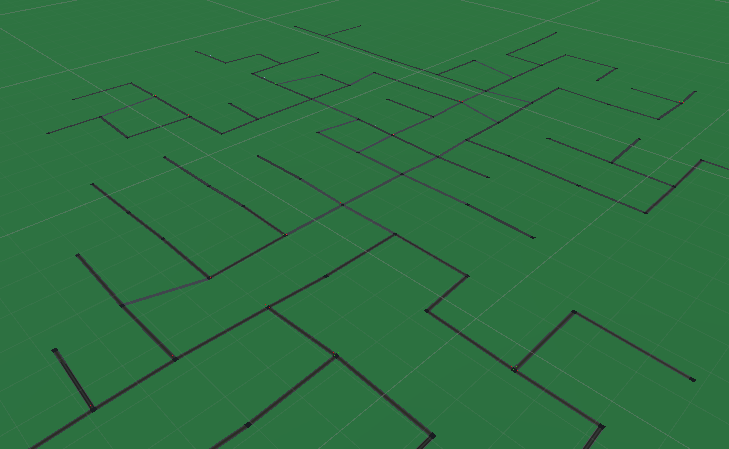
\includegraphics[width=\linewidth]{unitygraph.png}
\caption{Kép a generáló algoritmus eredményéről Unityben}
\label{fig:ugraph}
\end{figure}
